%% This section adds chapter 2
\section{Literature Review}

In order to understand startups and how AI-driven MVA development could happen, a literature study into the characteristics of startups and recent advancements in AI is needed. A process can be developed based on the insights found from the literature.

\subsection{Characteristics of a Software Start-up}
\textcite{giardinoSoftwareDevelopmentStartup2016} define software startups as "newly created companies with no operating history and oriented towards producing cutting-edge products." This definition reveals a few characteristics and constraints that affect how software startups operate. \textcite{suttonRoleProcessSoftwareJuly-Aug./2000} provides a list of these characteristics and constraints that are present in most software startups.

\begin{itemize}
	\item Young and inexperienced: Startups are new or relatively young and immature when compared to more mature and established software companies. They have very little accumulated experience or history.
	\item Limited resources: Startups usually have a focus on getting the product out, promoting it, and building alliances. Initial resources are used to achieve these activities.
	\item Multiple influences: There are many influences, such as investors, customers, partners, and competitors that all affect what the startup is doing and how. Startups are sensitive to different influences in the early stages of the company.
	\item New technologies and markets: Startups are more likely to adopt new technologies and trying to get into new markets. Developing technologically innovative products often requires cutting-edge tools and techniques.
\end{itemize}

\citeauthor{suttonRoleProcessSoftwareJuly-Aug./2000} argues that software startups do not often consider software processes. Because of their youth and immaturity, startups often do not have the foundations required for established processes. These foundations include "a historical record of experience, infrastructure for process instantiation and improvement, and repeatable and predictable practises." According to \citeauthor{suttonRoleProcessSoftwareJuly-Aug./2000}, process issues need to be solved and prioritized based on the startup's needs and the resources it has available.

\subsection{Software Architecture Design Process}
It is useful to understand what has been the more traditional software architecture design process before replacing them with AI tools or adding new ones into the mix. In their paper \cite{hofmeisterGeneralModelSoftware2007} present a general model derived from the industry. They selected multiple methods including Attribute-Driven Design, 4 Views, Rational Unified Process 4+1 views and a few others. They extracted the commonalities from these different methods to find the general model of architecture design.

The model by \citeauthor{hofmeisterGeneralModelSoftware2007} is presented in figure \ref{fig:Architecture_design_activities_hofmeister}

\begin{figure}[htbp]
	\centering
	\pdftooltip{%
		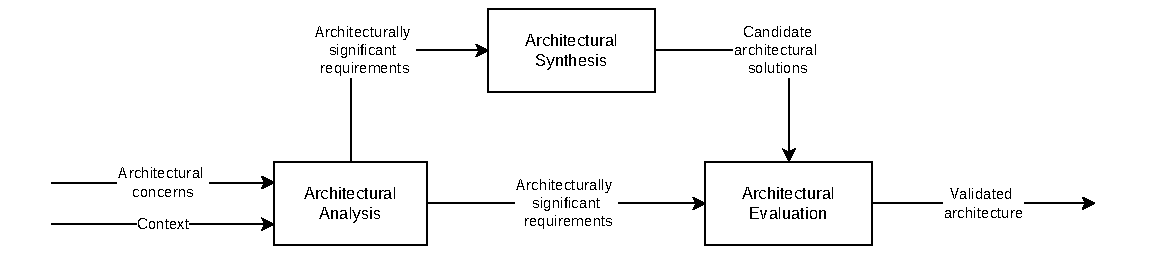
\includegraphics[width=\textwidth]{figs/Architectura_design_activities_hofmeister.pdf}%
	}{Figure showing the phases in a general software architecture design process. These phases include architectural analysis, architectural synthesis, and architectural evaluation.}
	\caption{A general model of software architecture design process.}
	\label{fig:Architecture_design_activities_hofmeister}
\end{figure}


\subsection{AI-driven Software Engineering}
Since LLMs have started to emerge, researchers have been trying to stay on top of the development. Plenty of studies have been made to find how LLMs can be used and what are their possibilities and limitations. Researchers, businesses, and developers try to find, how these tools can be best used to make software design and development more efficient and how developers' productivity can be increased.

Since the field of generative AI and LLMs is innovating very rapidly, it has to be noted that new tools are emerging fast and previous limitations can be overcome in a short moment. The research might struggle to keep up with such fast innovation.

\textcite{terragniFutureAIDrivenSoftware2025} write about the future of AI-driven software engineering. They argue that LLMs aren't going anywhere. They expect software engineers to continue to use these tools in the future. In their study, \citeauthor{terragniFutureAIDrivenSoftware2025} present a model for how AI could be integrated into every step of software development. Their vision for how software engineers and AI will work in a very close relationship is presented in figure \ref{fig:AI_in_development_process_terragni}.

\begin{figure}[htbp]
	\centering
	\pdftooltip{%
		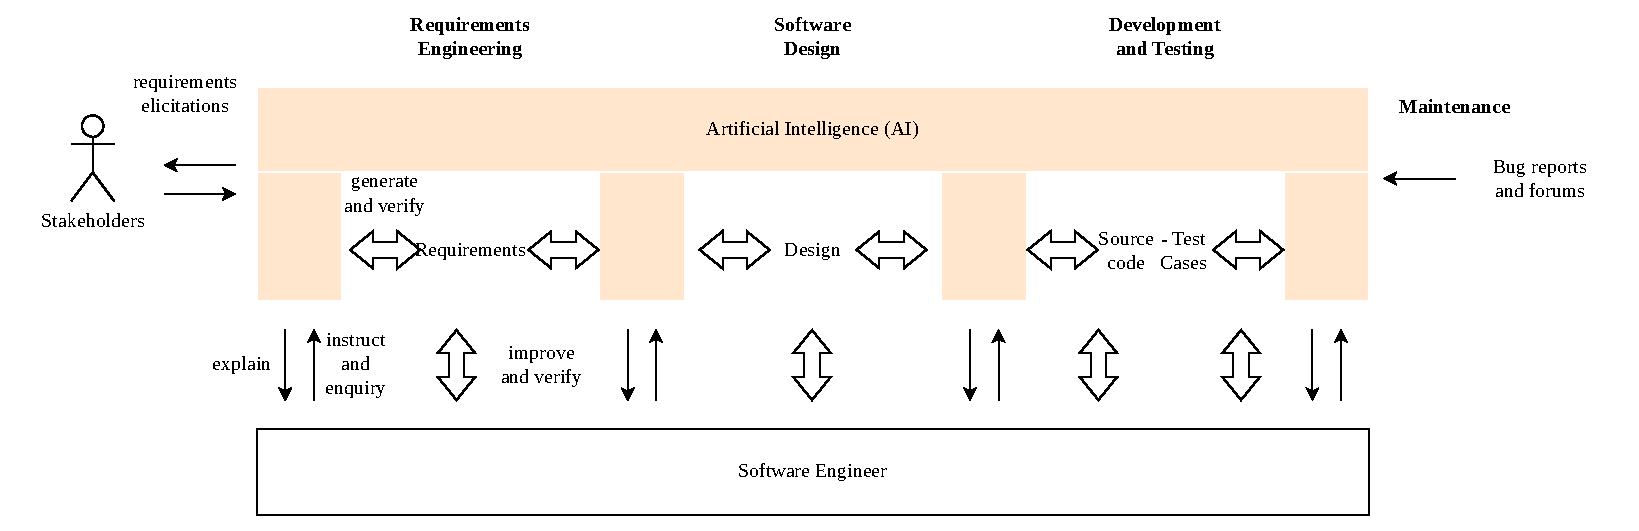
\includegraphics[width=\textwidth]{figs/AI_in_development_process_terragni.pdf}%
	}{Figure showing how AI will be integrated into software development process parts elicitation, requirements engineering, design, development, testing, and maintenance.}
	\caption{AI integration into software development process.}
	\label{fig:AI_in_development_process_terragni}
\end{figure}

In figure \ref{fig:AI_in_development_process_terragni} \citeauthor{terragniFutureAIDrivenSoftware2025} picture the communication between the AI and the software engineer in every part of the development process. At every stage, the engineer will instruct and enquiry the AI, which will in turn explain what it is doing. The AI then generates and verifies an artifact, for example the requirements. The software engineer then improves and verifies the artifact. This repeats in the stages design, and development and testing, which produce artifacts design, source code, and test cases. After the development process is finished, there is the maintenance stage where bug reports and forum discussions are fed into the AI, which will do the maintenance work in collaboration with the software engineer.

\subsection{Generative AI as an Architectural Assistant}
Generative AI tools, like LLMs have proved to be useable in providing assistance to software engineers. The rapid development of the models creates new possibilities and capabilities for software engineers to apply the models in traditional software development processes. There are predictions that AI tools could completely take over some tasks in the development process. \parencite{welshEndProgramming2023}

\textcite{cervantesLLMsAssistantsSoftware2026} argue that Generative AI and LLMs allow users to "rapidly identify, compare, and explore design alternatives". This would speed up the architecture design process and allow for faster ideation, iteration and software development. Based on their research they argue, that humans are still needed to make final architectural decisions, but this process can be helped by LLMs. LLMs can stimulate ideas, raise discussion, and even give feedback and act as a sounding board.

In their research, \citeauthor{cervantesLLMsAssistantsSoftware2026} found that LLMs can be very useful in divergent thinking. That means generating many ideas or solutions to the problem at hand. On the other hand, LLMs aren't that good at convergent thinking, which is putting those different ideas together. In practise this could mean, that the architect uses LLMs to quickly generate multiple solutions and enumerate their pros and cons. Then the architect can eliminate unsuitable solutions and make quicker decisions. This way "the architect's time can be spent in detailed analysis and comparison of a set of design concepts that both cover the horizon of possibilities and have been vetted, at least in part."

Another study found that AI tools greatly increase the productivity of developers. \textcite{amasantiImpactAIGeneratedSolutions2026} conducted a study on the impact of AI tools and found that 45\% of the survey participants had increased productivity when using AI tools. The productivity increased over 35\% which is a very significant percentage. \citeauthor{amasantiImpactAIGeneratedSolutions2026} argue that everyone who wants to stay competitive in the software industry must use AI tools. They also found that using AI generated code does not erode the quality of software architecture significantly.

The same study also found that AI can suggest architectural designs that are adequate. However, architects with less experience would most likely struggle to assess if the solutions are useable. AI also does not manage to offer suitable solutions when faced with larger and more complex problems. When AI works on these harder problems, it produced significantly lesser quality code than humans. This leads to a codebase, which is not easy to maintain and integrate. \citeauthor{amasantiImpactAIGeneratedSolutions2026} argue that software engineers are needed to synthesise the solutions into systems that are already well-architected. They think that "architecture skills are highly needed in the age of AI."

A recent literature review \parencite{espositoGenerativeAISoftware2026} found that LLMs can help software architects a lot in different parts of software development. The SALC phases where they are most often used are requirement-to-architecture (40\%) and architecture-to-code (32\%). Requirement-to-architecture phase is also used in the MVA design process. The study found that most used languages are Java (13\%), JavaScript, Python, UML, and Natural Language (NL). A significant number of research papers did not include the programming language of the use case. \citeauthor{espositoGenerativeAISoftware2026} argue that this makes it harder to analyze how LLM use cases and performance in different technology stacks. They also found that there are no clear best practices or guidelines. Even though prompt engineering, fine tuning and other strategies have been researched, no consensus has been found on how to effectively use GenAI in software architecture tasks.


\subsection{AI in Requirements Engineering}
A particularly interesting study \parencite{tagliaferroLeveragingLLMsAutomate2025} was made to research how LLMs can be used to produce UML component diagrams from informal NL descriptions. \citeauthor{tagliaferroLeveragingLLMsAutomate2025} argue that their approach is useful in the early stages of developing a new software. Their approach allows developers to produce an architecture for the system immediately without a thorough, often time-consuming requirements analysis. However, in their study they directly generated UML diagrams from the software description. It could be useful to include other steps in the process to achieve better results.

\textcite{calamoUserStoriesArchitectures2026} tried a different approach. In their study, they used a custom LLM-based framework, ArchiLLM, to generate an architecture from user stories. ArchiLLM developed a microservice-based architecture. After that, it generated the code for the application. They designed ArchiLLM to introduce a step between code generation and requirements, since LLMs itself don't have architectural vision. This leads to LLMs oversiplifying users request's or generating code doesn't work as the user wanted. \citeauthor{calamoUserStoriesArchitectures2026} introduce a new, important step where LLM designs an architecture before generating any code.

In their framework, \citeauthor{calamoUserStoriesArchitectures2026} used different agents, such as Microservice Extracting agent, Context Retrieval agent, and Architecture Generator agent. The results of the study suggest that the approach used in ArchiLLM has potential in some areas to increase effectiveness, efficiency, and code development. Some limitations concern LLMs inability to picture more complex software. In some cases, ArchiLLM tried to generate too complicated microservices. \citeauthor{calamoUserStoriesArchitectures2026} would also like to introduce humans to the process to critique, suggest modifications, answer LLM's questions and revise the requirements.

\subsection{LLMs in Generating Architecture Diagrams}
\textcite{tagliaferroLeveragingLLMsAutomate2025} used ChatGPT to generate a PlantUML diagram from informal software specifications. Instead of directly asking for a graphical output, they asked the LLM to generate a PlantUML diagram, which is a textual model, since it lead to better results. Their results show that LLMs generally generated diagrams, that were correct syntactically and included the elements that were part of the informal specifications. However, the diagrams included oversimplifications and lacked elements specific to certain domains. \citeauthor{tagliaferroLeveragingLLMsAutomate2025} argue that these diagrams can work as helpful starting points for the software architecture design process, "particularly if paired with post-processing automatic refinement techniques."

Another study \parencite{ramachandranTransformingSoftwareArchitecture2025} researched how AI tools can "enhance productivity, ensure design consistency, and support architectural decision-making." They argue, that many diagrams use repetitive patters that could be created automatically. In their study, they utilized LLMs to generate UML diagrams. The results of the study show, that AI generated diagrams were better than those generated by humans. Even though LLMs had difficulties with class diagrams, they performed well with use case diagrams, sequence diagrams, and state diagrams.

\subsection{Quality Assessment and Validation of Architecture}

Research has been conducted on how LLMs could automatically assess if architecture diagrams are good quality. A study by \textcite{deoliveiraLLMBasedQualityAssessment2026} used AI to evaluate diagrams according to five main criteria: clarity, consistency, completeness, accuracy, and level of detail. The study found that some quality issues can be recognized by LLMs. Especially issues with inconsistencies or missing elements were found. However, LLMs might misinterpret the choices made in the design without context or they might overestimate omissions, which requires humans to oversee the process. \citeauthor{deoliveiraLLMBasedQualityAssessment2026} present a set of guidelines that can be used to improve the effectiveness of generative AI. This set includes consolidating artifacts, using high-quality images, prompting explicitly, and encouraging step-by-step reasoning. Following these guidelines will ensure better
"alignment between visual and textual architectural representations."

One possibility to assess the quality of AI generated architecture is to look at the design rationale (DR). DRs are an important part of architecture design. However, often DRs are not collected adequately \parencite{tyreeArchitectureDecisionsDemystifying2005}. \textcite{zhouUsingLLMsGenerating2025} argue that LLMs can be used to bridge this gap. In the study they created prompt templates and developed a system to generate design rationale for architecture decisions. The results show that LLM generated DRs managed to capture most of the key points when making architecture decisions. LLMs usually provides a more varied range of different arguments and perspectives than humans do. However, the DRs often lack specific details and project experience. It is also very hard to reduce the proportion of "uncertain" arguments using the prompting strategies the study used.

\subsection{Challenges and Risks of AI in Architecture Design}
Using GenAI and LLMs in architecture design also introduces some risks. In their literature study, \textcite{espositoGenerativeAISoftware2026} found that "model precision, hallucinations, ethical aspects, privacy issues, lack of architecture-specific datasets, and the absence of sound evaluation frameworks" are some of the most pressing issues and challenges at the moment. 15\% of the studies reviewed found LLM accuracy to be a challenge. 9\% found hallucinations and 7\% ethical concerns. 9\% of the studies they reviewed did not mention challenges, which "indicate gaps in recognizing and addressing limitations of LLMs in software architecture."

\textcite{ozkayaApplicationLargeLanguage2023} argues that despite LLMs frequently make significant improvements, there are still topics to be cautious about. \citeauthor{ozkayaApplicationLargeLanguage2023} points out data quality and bias concerns, privacy and content ownership concerns, environmental concerns, and explainability and unintended consequence concerns. For example, the concerns about data quality and bias can lead to buggy code being generated, if not taken into account. The quality of the training data used to train the language model can contribute to the performance of the model. However, \citeauthor{ozkayaApplicationLargeLanguage2023} also argues that there are many areas of software engineering that can significantly benefit from LLMs.

\clearpage  % This command will start the next section from the new page
